\subsection{Análise descritiva de dados}

O processo de análise descritiva de dados, incluindo distribuições de frequência, técnicas de visualização de dados e medidas resumo

Descrever e encontrar o que há nos dados.
Ao passo que no futuro pode ser implementar algoritmos de mineração que buscam conclusões que extrapolam os dados e permitem inferir predições.
Portanto, analise descritiva descreve as características dos dado e a mineração geralmente usada em análise mais abrangentes visando a predição.
Entretanto, precisa ficar atento com falsas correlações e predições dos dados.

Análise descritiva permite descrever a distribuição e a correlação dos atributos, utilzando medidas estatísticas, como distribuição de frequência, tendência central e visualização gráfica, sendo para atributos univariada e para bivariada relações entre atributos.

\subsubsection*{Processo}

\paragraph*{Distribução de frequência}

\paragraph*{Técnica de visualização}
\begin{itemize}
    \item Histograma
    \item Polígonos de frequências
    \item Ogiva
    \item Gráfico de Pareto
    \item Gráfico de setores
    \item Gráfico de dispersão - scatterplots
\end{itemize}

\paragraph*{Medidas de tendência central, variação e associação}

\begin{figure}[!htp]
    \centering
    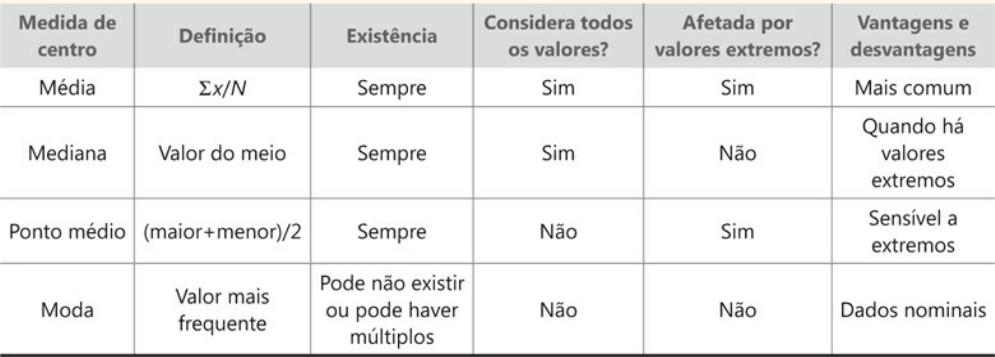
\includegraphics[scale=.4]{../img/estatistica/tendencia-central.png}
    \caption{Tendência Central}
    \label{img:tendencia_central}
\end{figure}

\begin{itemize}
    \item Moda
    \item Mediana
    \item Ponto Médio
          \begin{equation} \label{eq:ponto_medio}
              \frac{maior - menor}{2}
          \end{equation}
    \item Média amostral
          \begin{equation} \label{eq:media_amostral}
              \bar{x} = \frac{1}{n} \sum^{n}_{i=1} x_i
          \end{equation}
    \item Média populacional
          \begin{equation} \label{eq:media_populacional}
              \mu = \frac{1}{n} \sum^{n}_{i=1} x_i
          \end{equation}
    \item Média de distribuição de frequências
          \begin{equation} \label{eq:media_distribuicao_frequencia}
              \bar{x} = \frac{\sum^{n}_{i=n} f_i * x_i} {\sum^{n}_{i=n} f_i}
          \end{equation}
    \item Média ponderada
          \begin{equation} \label{eq:media_ponderada}
              \bar{x} =
              \frac{\sum^{n}_{i=n} (w_i * x_i)}
              {\sum^{n}_{i=n} w_i}
          \end{equation}
    \item Média geométrica
          \begin{equation} \label{eq:media_geometrica}
              \bar{x} = (\Pi^n_{i=1} x_i)^{\frac{1}{n}}
          \end{equation}
    \item Média harmônica
          \begin{equation} \label{eq:media_harmonica}
              \bar{x} = \frac{n}{\sum^{n}_{i=1} \frac{1}{x_i}}
          \end{equation}
    \item Medidas de dispersão
    \item Amplitude
          \begin{equation} \label{eq:amplitude}
              amplitude = maior - menor
          \end{equation}
    \item Desvio Padrão
          \begin{equation} \label{eq:desvio_padrao}
              \begin{split}
                  s = \sqrt{\frac{1}{n-1} \sum^n_{i=1} (x_i - \bar{x})^2}
                  \\
                  \sigma = \sqrt{\frac{1}{n-1} \sum^n_{i=1} (x_i - \bar{x})^2}
              \end{split}
          \end{equation}
    \item Coeficiente de variação (CV)
          \begin{equation} \label{eq:coeficiente_variacao}
              CV = \frac{\sigma}{\mu} * 100\%
          \end{equation}
    \item \underline{Medidas de forma:}
          a assimetria~(Skewness) distribuição dos dados, pode ser nula( No Skewness) conhecido pela nomeclatura de curva sino, podendo receber descolamento positivo da assimetria~(Positive Skewness) ou negativa~(Negative Skewness).
          Assimetria é calculada da seguinte forma:
          \begin{equation} \label{eq:medidas_forma}
              \gamma = \frac{E(x - \bar{x})^3}{\sigma^3}
          \end{equation}
    \item \underline{Curtose Kurtosis}
          é uma medida de dispersão que caracteriza o pico ou achatamento da curva da função de distribuição normal.
          \begin{equation} \label{eq:curtose_kurtosis}
              \beta = \frac{E(x - \bar{x})^4}{\sigma^4}  -3
          \end{equation}
    \item Medidas de posição relativa
    \item Quartils e boxplot
          \begin{itemize}
              \item Medida de associação
              \item Covariância
                    \begin{equation} \label{eq:covariancia}
                        cov(x,y) = \frac{1}{N} \sum^{N}_{i=1} (x - \bar{x}) (y - \bar{y})
                    \end{equation}
          \end{itemize}
    \item \underline{Coeficiente de correlação de Pearson:}
          mede a dependência linear entre os atributos de forma linear~\footnote{https://statistics.laerd.com/statistical-guides/pearson-correlation-coefficient-statistical-guide.php}.
          \begin{equation} \label{eq:pearson}
              \rho(x,y) = \frac{cov(x,y)}{\sigma(x) * \sigma(y)}
          \end{equation}
\end{itemize}


\begin{table}
    \centering
    \caption{Coeficiente de correlação de Pearson}
    \begin{tabular}{c|l}
        \hline
        \textbf{Size of Correlation} & \textbf{Interpretation}                   \\ \hline
        $ |~0.90 - 1.00~| $          & Very high positive (negative) correlation \\ \hline
        $ |~0.70 - 0.90~| $          & High positive      (negative) correlation \\ \hline
        $ |~0.50 - 0.70~| $          & Moderate positive  (negative) correlation \\ \hline
        $ |~0.30 - 0.50~| $          & Low positive       (negative) correlation \\ \hline
        $ |~0.00 - 0.30~| $          & Negligible correlation                    \\ \hline
    \end{tabular}
    \label{tab:pearson}
\end{table}


\paragraph*{Visualização dos dados}

\begin{itemize}
    \item Medidas de resumo
    \item Medidas de tendência central
    \item Medida de dispersão
    \item Medida de forma distribuição
\end{itemize}
